\documentclass[12pt]{article}
\usepackage[margin=1.2in]{geometry}
\usepackage{amsmath}
\usepackage{graphicx}
\usepackage{caption}
\usepackage{subcaption}
\begin{document}
\title{COL334 - Assignment 1\\ Internet Architecture}
\author{Akshay Kumar Gupta\\\texttt{2013CS50275} \and  Barun Patra\\\texttt{2013CS10773} \and Haroun Habeeb\\\texttt{2013CS10225}}
\date{}
\maketitle
\noindent {\bfseries Q2a.} Variation of number of hosts on IIT-Delhi Wifi over the course of a week:\\
~
\\

{\centering{
{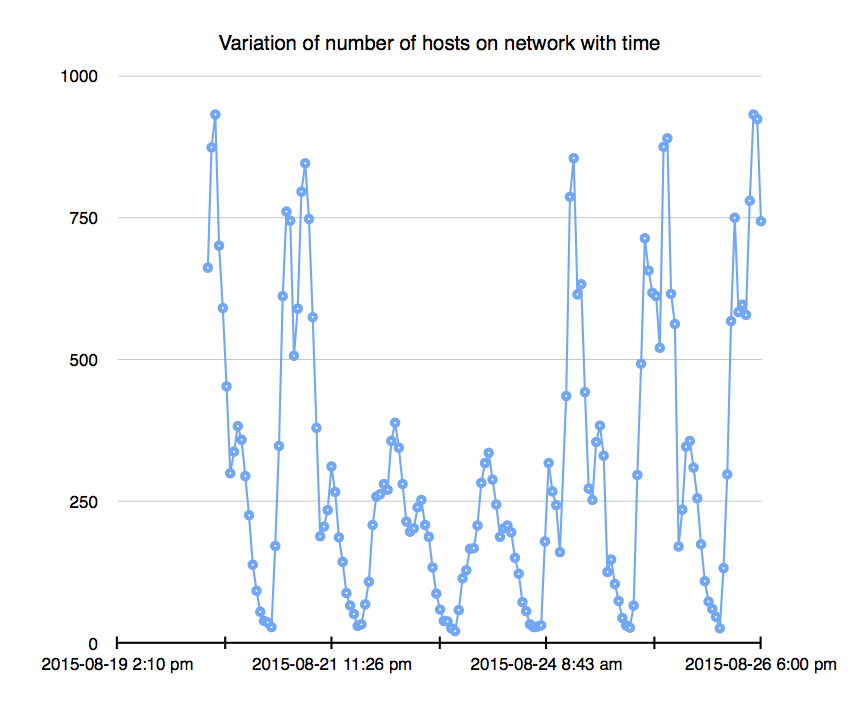
\includegraphics[scale=0.55]{../src/2aResults.png}
}
}}
~
\\
{\bfseries Q2b.} Running the nmap command on 10.192.46.*, 13 hosts were discovered. The IP addresses of the hosts were:
\begin{itemize}
\item 10.192.46.5
\item 10.192.46.14
\item 10.192.46.27
\item 10.192.46.29
\item 10.192.46.39
\item 10.192.46.48
\item 10.192.46.55
\item 10.192.46.63
\item 10.192.46.74
\item 10.192.46.89
\item 10.192.46.98
\item 10.192.46.104
\item 10.192.46.212
\end{itemize}
~\\
{\bfseries Q2c.} List of Gateways and DNS Servers used in different parts of the campus:
\begin{itemize}
\item Hostel LAN (Kumaon)
\begin{itemize}
\item Gateway : 10.243.144.1
\item DNS Servers : 10.10.1.2, 10.10.2.2
\end{itemize}
\item Bharti Wifi
\begin{itemize}
\item Gateway : 10.192.32.1
\item DNS Servers : 10.10.1.2, 10.10.2.2
\end{itemize}
\item Bharti LAN
\begin{itemize}
\item Gateway : 10.208.20.1
\item DNS Servers : 10.208.20.2
\end{itemize}
\item CSC
\begin{itemize}
\item Gateway : 10.235.13.1
\item DNS Servers : 10.8.2.3, 10.10.1.2
\end{itemize}
\end{itemize}
\end{document}